\documentclass{article}
\usepackage[utf8]{inputenc}
\usepackage{caption}
\usepackage{amsmath}
\usepackage{amssymb}
\usepackage{mathtools}
\usepackage{multicol}
\usepackage{graphicx}
\usepackage{wrapfig}
\usepackage{float}
\usepackage[makeroom]{cancel}
\usepackage{mhchem}
\usepackage{pst-plot}

\graphicspath{ {../images/} }

\renewcommand{\baselinestretch}{1.5} % line spacing
\newcommand{\fline}{\par\noindent\rule{\textwidth}{0.1pt}} % horizontal line (wide)

\title{Topic 8/18 Acids \& Bases\\8.1 Identifying Acids + Bases}
\author{Peter Zhang}

\begin{document}

\maketitle
\newpage
\tableofcontents
\newpage

% lesson 

\section{Overview}
\begin{enumerate}
\item identifying Acids + Bases
\item pH
\item Lewis Acids + Bases
\item $K_{a} + K_{b}$
\item pH curves
\end{enumerate}

\section{Theories of Acids + Bases}
\subsection{Lovoisier}
\begin{itemize} \item Acids must contain oxygen \item from basic tests + etc, as long as Oxygen was present similar properties began to show (for acids and bases) \item he was using a polyatomic form and also at the time, Oxygen was 'the thing' cuz it gave life etc \end{itemize}
\subsection{Arrhenius}
\begin{itemize} \item \ce{H+ + OH-} meant that there were acid and base \item This made identifying acids easier to identify \item Example: [\ce{HCl (aq) $\rightarrow$ H+(aq) + Cl-(aq)}] | All solutions must be aqueous \item He was right, but it's not the whole picture. \item This does not define all possible acids/bases! \item Bases are not just hydroxide ions, metal oxides, metal bicarbonates, etc all have 'basic' properties. \item Example: [\ce{NaOH(aq) -> Na+(aq) + OH-(aq)}] \end{itemize}
\subsection{Bronsted-Lowry}
\begin{itemize}
\item an acid will 'donate' a proton (\ce{H+}) [not actually talking about proton - only electrons move. Using proton is just stating that a positive charge will move] \item a base will accept the proton (\ce{H+}) \item Example: [\ce{NH3 - base}] Cannot be explained using Arrhenius - this is because it doesn't have any \ce{OH-} so cannot be base in Arrhenius. \item If we look at the nitrogen, we know that it can bond with another Hydrogen to form Ammonium (from ammonia). Since Nitrogen has an available position to create a coordinate covalent bond,  it can 'accept' a 'proton'.  \item We basically looking for a lone pair - for coordinate covalent bonds! \item This also relates to polyatomic compounds and ligands! \item \ce{CH3COOH -> CH3COO- + H+} (reactant is an acid) \item \ce{CH3COOH + NH3 $\rightleftharpoons$ CH3COO- + NH4+} \begin{figure}[H]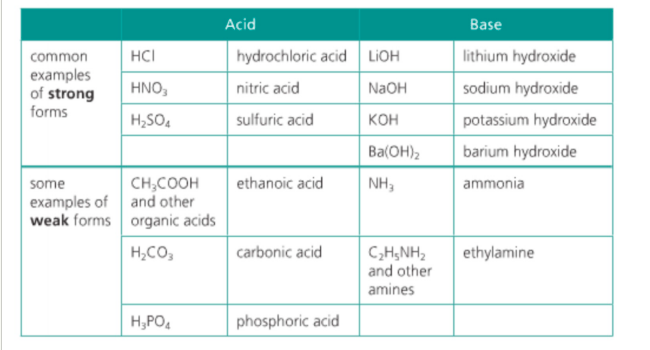
\includegraphics[width=\textwidth]{3.1fig1.png}\captionof{figure}{Strong and Weak Acids + Bases}\end{figure}
\item \textbf{conjugate base}: more likely to accept proton (remove proton from acid)  \item \textbf{conjugate acid}: more likely to donate proton (add a proton to base) \item Some molecules can be \textbf{amphiprotic} (can accept or donate protons) [\textbf{insert image -- from lesson slides about H2O and something something blah blah i dont know}]
\end{itemize}

\subsection{Solutions and Stuff}
\begin{itemize} \item If solutions are aqueous we tend to break them up into their ions: \\\ce{HCl(aq) + K(s) $\rightleftharpoons$ KCl(aq) + \frac{1}{2}H2(g)} \item Basically if one is behaving acidic, the other must behave as a base. Base mst be recognized through Arrhenius, Lewis-Base or Bronsted-Lowry. \item If none of these requiremenst are met, then this means you cannot apply acid-base equations to the reaction.  \\\begin{center}
\begin{align*}
\ce{HCl(aq) + K(s)} &\rightleftharpoons \ce{KCl(aq) + \frac{1}{2} H2(g)}\\
\ce{H+(aq) + K(s)} &\rightleftharpoons \ce{K+(aq) + \cancel{Cl-(aq)} + \frac{1}{2}H2(g)}\\
\ce{H+(aq) + K(s)} &\rightleftharpoons \ce{K+(aq) + \frac{1}{2}H2(g)}
\end{align*}
\end{center}

\item Can last for changes in pH using chemical indicators or litmus paper\\ex: \ce{HIn_{colour A} $\rightleftharpoons$ H+ + In-_{Colour B}}
\item If you mix more acid in, it shifts towards Colour A (reactants) and vice verse
\end{itemize}

\pagebreak
\subsection{Overview}
\begin{enumerate}
\item Add proton to base = conjugate acid
\item Remove proton from acid = conjugate base
\item \textbf{ONLY ACIDS react with metals} | NOT BASES | transition metals can react with some bases (NH4) as ligands to create complex ions
\end{enumerate}













\end{document}